\DocumentMetadata{
    lang = en-US,
    tagging = on,
    pdfstandard = ua-2
}
\documentclass[11pt]{article}
% 1. Colors & Graphics
\usepackage{xcolor}
\usepackage{tikz}
\usepackage{graphicx}
\usetikzlibrary{arrows.meta,positioning,calc}
\usepackage{ccicons}

% 2. Lists & Text Formatting
\usepackage[normalem]{ulem}

% 3. Tables
\usepackage{booktabs}
\usepackage{tabularx}
\usepackage{placeins}

% 4. Bibliography & Citations (must be loaded before hyperref)
\usepackage[authoryear,round]{natbib}

% 5. Hyperlinks (almost always loaded near the very end)
\usepackage{hyperref}
\usepackage{xurl}
\hypersetup{hidelinks}

% 6. Post-hyperref patches
\usepackage{breakcites}

%\renewcommand{\footnoterule}{} % Uncomment to pass VerePDF UDL/accessibility tests

\hypersetup{
    pdftitle={AI Fundamentals: How AI Works, How It Is Changing, and How to Evaluate It},
    pdfauthor={Gregory Anderson},
    pdfsubject={A Primer for Faculty and Staff},
    pdfdisplaydoctitle=true
}
\pagestyle{plain}

\title{
    \textbf{Making Sense of AI}\\[4pt]
    \large How AI Works, How It Is Changing, and How to Evaluate It\\
    \textit{A Primer for Faculty, Students, and Staff}%
  \footnote{
  AI applications (ChatGPT, Claude, and Gemini) assisted with brainstorming, drafting, editing, and developing illustrations. The document's conceptual framing, selection of examples, fact checking, and substantive revisions were directed by the author, who retains responsibility for all of its content.
  For reflections on the AI-assisted writing process, see Section~\ref{sec:afterword}.}
}

\author{
    Gregory Anderson\thanks{Licensed under \ccbysa
  \href{https://creativecommons.org/licenses/by-sa/4.0/}{CC BY-SA 4.0}.
  Source files and latest version:
  \url{https://github.com/gregorywanderson/ai_fundamentals}.}\\
    {\small Department of Physics}\\
    {\small Northeastern Illinois University}
}

\date{\today}
\begin{document}

\maketitle

\begin{abstract}
This document introduces artificial intelligence to faculty, students, and staff across academic disciplines. It explains how contemporary AI systems are trained and generate responses, and distinguishes AI models from the applications and agents built on them. It then examines why AI capabilities have advanced rapidly, why progress varies across tasks, and how that progress is measured. Finally, it explains why capability does not guarantee reliability. Two recurring examples---a historian's question about the French Revolution and an environmental scientist's question about ozone trends in Chicago---illustrate the document's central point: the important question about an AI response is not whether it sounds convincing, but what information and methods produced it and how its conclusions can be checked. The document focuses on foundational understanding rather than classroom pedagogy or institutional policy. It is intended to support AI literacy training and to serve as a reference. 
\end{abstract}

\clearpage
\tableofcontents

\clearpage
\section*{Learning Outcomes}

\begin{itemize}
\item\textbf{Identify} and distinguish artificial intelligence, machine learning, deep learning, generative AI, large language models, and foundation models, using examples from familiar applications.
\item\textbf{Explain}
how contemporary AI models are trained and generate responses, including the roles of neural networks, optimization, computing hardware, pretraining, post-training, and inference.
\item\textbf{Differentiate}
  AI models, applications, and agents, and explain how their capabilities and limitations depend on training, access to information, external tools, and human oversight.
\item\textbf{Explain}
the main drivers of AI progress (model design, computation, and data), why that progress is uneven across tasks, and how to interpret benchmark evidence while recognizing its limitations.
\item\textbf{Explain} why AI-generated information can be incorrect or incomplete, and select verification practices appropriate to the task and its consequences.
\end{itemize}

%\tableofcontents
\section*{Introduction}

\noindent\textbf{A Tale of Two Queries.}
A history professor asks an AI assistant to explain the causes of the
French Revolution. It produces an articulate account of fiscal crisis,
social inequality, and political ideas. Did it consult historical sources,
or did it generate an explanation from patterns and associations acquired during training?

A second professor asks an AI assistant how ground-level ozone in the Chicago region
has changed over the past twenty years.
The assistant may retrieve EPA monitoring data and calculate trends, but selecting an appropriate measure of ozone and evaluating the data still require scientific judgment. In either case, the crucial question is not simply whether the response sounds convincing, but what information and methods the system actually used and how its conclusions can be checked.

These two cases will help distinguish what a model has learned from
what an application can actually verify and do. The questions also
arise in education, business, and many other disciplines.

\section{What Is Artificial Intelligence?}

\textbf{Artificial intelligence (AI)} is a broad field of computer
science concerned with developing systems capable of performing tasks
that ordinarily require aspects of human intelligence. Examples include
recognizing images, understanding language, identifying patterns,
making predictions, solving problems, and planning actions. The term
encompasses many different technologies, some of which have been in
widespread use for decades.

Definitions of AI systems are not entirely uniform. The 
OECD\footnote{The Organisation for Economic Co-operation and
Development (OECD) is an international organization that conducts
research and develops policy recommendations and international
standards.}
describes an AI system as one that infers from its inputs how to produce outputs
such as predictions, content, recommendations, or decisions. This
definition does not require learning from data, and the boundary between
AI and simpler conventional software is not always sharply defined
\citep{OECD2024AIDefinition}.

\textbf{Machine learning (ML)}
is a branch of AI in which computers
learn patterns and relationships from data rather than relying
exclusively on explicitly programmed rules. A conventional
calculator, for example, follows programmed mathematical
procedures to perform arithmetic. It does not learn how to
multiply by examining examples of multiplication.

In contrast, a machine learning algorithm learns from training data by adjusting the parameters of a mathematical model to improve its performance on a particular task. Once trained, the model can apply what it has learned to new data. For example, an email spam filter can learn to distinguish legitimate messages from spam by analyzing examples of both.

Most contemporary AI applications use some form of machine learning,
although not all AI systems do. Earlier approaches to AI relied
heavily on explicitly programmed rules, logical inference, and
expert systems.

\textbf{Deep learning} is a form of machine learning that uses artificial neural networks with multiple layers. These networks consist of interconnected computational units that process information, with adjustable connections that are modified during training. Deep learning is used in applications such as speech recognition, image classification, and many contemporary generative AI systems.

\textbf{Generative AI} is a category of AI that produces new content,
including text, images, audio, video, and computer code. Unlike
systems designed primarily to classify information or make predictions
about existing data, generative AI models learn statistical patterns
that allow them to produce new outputs in response to instructions
or other inputs. Examples include ChatGPT, Claude, Gemini, and AI
image-generation systems.

\textbf{Large language models (LLMs)} are a class of machine learning
models trained on enormous collections of text and other data to
process and generate language. Most contemporary LLMs use a neural
network architecture called the \emph{transformer}. During training,
they learn statistical relationships among words, symbols, and
other elements of language, represented as \emph{tokens}. A common
training objective is to predict the next token in a sequence.
This process enables LLMs to generate coherent text, answer
questions, translate languages, summarize documents, and perform
many other tasks.

LLMs are central to many generative AI applications, but they are
not synonymous with generative AI. Models that generate images,
audio, or video may use different architectures, although
increasingly these capabilities are combined in \emph{multimodal
models} that can process or generate several kinds of information
\citep{Bommasani2021}.
In some multimodal models, images are divided into patches and represented
numerically, much as text is represented by tokens. Other generative
systems, including many image generators, use \emph{diffusion}: they learn
to generate images by progressively removing noise from an initially
random pattern \citep{Ho2020Diffusion}.

\textbf{Small language models (SLMs)} are language models with relatively few parameters compared with the largest LLMs. They generally require less computing power and memory, making them suitable for specialized applications and deployment on personal computers or mobile devices. Although they may have more limited general capabilities, SLMs can perform competitively with larger models on particular tasks.

\textbf{Foundation models} are large machine learning models
trained on broad datasets that can be adapted to perform many
different tasks. Rather than developing a separate model from
scratch for each application, developers can use a foundation
model as the basis for more specialized systems. Adaptation
may involve additional training (\emph{fine-tuning}), providing
task-specific instructions, or supplying relevant information
at the time the model is used. Large language models are an
important category of foundation models, but foundation
models can also process images, audio, video, and other forms
of data \citep{Bommasani2021}.

For example, Google's \textbf{BERT} \citep{Devlin2019BERT} is a pretrained language model that can
serve as the starting point for specialized systems that classify
emails as spam, identify whether a review is positive or negative,
recognize names and places in text, or find answers in a supplied
passage. Developers can adapt the same underlying model for these
different tasks rather than train a new one from scratch. BERT
illustrates a foundation model used mainly to analyze existing
text, rather than to generate new passages.
Google began incorporating BERT into its search engine in 2019 to improve its interpretation of search queries. Thus, many people encountered applications of transformer-based language models well before the emergence of ChatGPT \citep{Google2019BERTSearch}.


Other foundation models are also generative. For example, a
pretrained large language model can underlie applications for
tutoring, summarizing documents, and assisting with computer
programming. Such applications may specialize the model through
instructions, additional training, or access to external information.
Thus, many contemporary LLMs occupy the overlap between foundation
models and generative AI in Figure~\ref{fig:ai_relationships}.

\textbf{Frontier models} are the most capable general-purpose
models available at a given time, typically developed by a small
number of companies with access to very large computing resources
\citep{StanfordHAIFrontier}. The term is relative: today's frontier
model may be an ordinary one within a year or two. Frontier models
are generally foundation models, but most foundation models are not
at the frontier. Some regulations define frontier models by the
amount of computation used to train them rather than by capability.

\subsection{Relationships Among AI Technologies}

These terms describe different aspects of AI and should not be
treated as interchangeable. Artificial intelligence is the
broadest category, encompassing both rule-based systems and
systems that learn from data. Machine learning is a subset of
AI. \textbf{Deep learning} is a form of machine learning
using multilayer artificial neural networks.

Foundation models describe broadly adaptable models; generative AI
is defined by what a system produces. These categories overlap but
are not interchangeable. The figure summarizes the principal
relationships for contemporary systems.


\begin{figure}[htbp]
\centering
\begin{tikzpicture}[font=\small,scale=0.83,transform shape,
alt={Nested regions show AI containing machine learning, which contains deep learning. Within deep learning, foundation models and generative AI are overlapping categories, with many modern large language models belonging to both.}]

  % Artificial intelligence
  \draw[rounded corners=10pt, thick, fill=gray!7]
    (0,0) rectangle (13,8);
  \node[anchor=west,font=\bfseries]
    at (0.25,7.65) {Artificial intelligence (AI)};

  % Machine learning
  \draw[rounded corners=9pt, thick, fill=green!8]
    (0.75,0.7) rectangle (12.35,7.15);
  \node[anchor=west,font=\bfseries]
    at (1.0,6.75) {Machine learning (ML)};

  % Deep learning
  \draw[rounded corners=8pt, thick, fill=yellow!12]
    (1.5,1.45) rectangle (11.55,6.2);
  \node[anchor=west,font=\bfseries]
    at (1.75,5.8) {Deep learning};

  % Foundation models
  \draw[thick,blue!70!black,
        fill=blue!25,fill opacity=0.32]
    (5.6,3.65) ellipse
    [x radius=3.15,y radius=1.45];

    % Generative AI
   \draw[thick,red!70!black,
      fill=red!25,fill opacity=0.30]
    (8.7,3.55) ellipse
    [x radius=2.8,y radius=1.43];

  % Labels
  \node[font=\bfseries,align=center]
    at (4.35,4.05)
    {Foundation\\models};

  \node[font=\bfseries,align=center]
    at (9.85,3.95)
    {Generative\\AI};

  % Intersection
  \node[draw,rounded corners=3pt,
        fill=white,inner sep=4pt,align=center]
    at (7.3,3.35)
    {Many modern\\LLMs};

  \node[font=\scriptsize,anchor=west]
    at (2,1.83)
    {Not all AI is generative;
     not all generative AI uses foundation models.};

\end{tikzpicture}

\caption{Conceptual relationships among AI technologies.
AI, machine learning, and deep learning form a hierarchy.
Foundation models and generative AI overlap, but neither
category is strictly a subset of the other. The diagram
is schematic rather than a complete classification.}
\label{fig:ai_relationships}
\end{figure}

These relationships are important because the capabilities,
limitations, and risks of an AI application depend partly on
the models and methods underlying it \citep{Bommasani2021}.

\FloatBarrier
\subsection{AI in Everyday Life}

Most faculty, students, and staff have encountered increasingly sophisticated computing
technologies through everyday writing tools. These familiar examples
help distinguish conventional programming, machine learning, and
generative AI. The tasks are different, even when a single application
performs several of them.

\paragraph{Writing Assistance: From Rules to Generation}

\begingroup
\setlength{\leftmargini}{1em}
\begin{itemize}

\item \textbf{Identifying misspelled words:}
A conventional spell checker can compare words with a dictionary and
flag those it does not recognize. This requires no machine learning.

\item \textbf{Suggesting spelling corrections:}
Identifying an error is different from selecting a replacement. A
program can propose words with similar spellings using explicit
algorithms; a statistical or machine-learning system can also consider
word frequency and the surrounding sentence.

\item \textbf{Checking grammar:}
A rule-based checker can flag certain grammatical constructions.
More sophisticated systems use patterns learned from language to
identify errors that depend on context. For example, ``Their going
to class'' contains no misspelled words, but \emph{Their} should be
\emph{They're}.

\item \textbf{Automatic formatting:}
A word processor may turn a line beginning with ``1.'' into a numbered
list or capitalize the beginning of a sentence. Such behavior can be
implemented with programmed rules rather than AI.

\item \textbf{Predictive text:}
A phone or email application suggests a word or phrase based on the
text already entered. These suggestions can use statistical language
models or machine learning.

\item \textbf{Generating and revising text:}
A contemporary generative AI assistant can draft paragraphs, summarize
material, or rewrite prose in response to instructions. Unlike a tool
that merely corrects spelling or grammar, it may also change the
substance of what is being said.
\end{itemize}
\endgroup

These distinctions describe \emph{tasks}, not mutually exclusive types
of software. A spelling suggestion might come from a simple algorithm
or a language model, and a modern word processor may combine both.
The progression from predicting a word to generating extended text
provides a familiar point of entry to the language models discussed
in Section~\ref{sec:how-models-work}.

\paragraph{Other Familiar Applications}

AI is not limited to writing. Email spam filters can learn
to classify messages; recommendation systems suggest videos,
music, or products; navigation applications predict travel
times; and speech recognition converts spoken language into
text. Other examples include image recognition in smartphone
photography, fraud detection in financial transactions,
AI-assisted programming, image generation, and
educational tutoring tools. These applications use different
combinations of conventional algorithms, machine learning, and
generative models.

\medskip

\noindent
\textbf{Key distinction:}
AI describes a broad collection of computational approaches;
machine learning describes methods for learning from data;
generative AI describes systems capable of producing new content;
and LLMs are a particularly influential family of models
underlying contemporary language-based generative AI.

\section{How Do AI Models Work?}\label{sec:how-models-work}

Modern AI models learn statistical relationships from data.
Unlike conventional computer programs, in which developers
explicitly specify the rules governing a computation, machine
learning systems adjust the parameters of mathematical models
through a process called \emph{training}. The resulting models
can apply the patterns they have learned to new inputs.

For contemporary large language models, training commonly occurs in two broad stages: pretraining and post-training. Pretraining is the initial stage, in which a model develops general capabilities from large and diverse datasets. Post-training builds on this foundation, using additional training to refine the model's capabilities and behavior. Despite their names, these are not processes that occur before and after a separate training stage; both are forms of training.

Return to the history professor's question. How can a model
produce a fluent account of the causes of the French
Revolution, and why does that account still need checking?
The answer depends on the distinction between
\emph{training} a model and \emph{using} one.

\subsection{Training as an Optimization Problem}\label{sec:optimization}

Consider the \emph{traveling salesman problem}: a traveler must
visit a collection of cities and return to the starting point
while minimizing the total distance traveled. For eight cities,
there are already $(8-1)!/2 = 2{,}520$ distinct round-trip routes (counting a
route and its reverse as the same). Trying every route quickly
becomes impractical as the number of cities grows. One strategy
is to begin with a route, make a small change, and keep the
change if it shortens the journey. Repeating this procedure can
find a good route, although it may stop at a \emph{local minimum}:
a route that cannot be improved by the particular small changes
being considered, even though a shorter route exists elsewhere.

Training a neural network is also an \emph{optimization} problem.
Instead of minimizing distance, it seeks weights that minimize
a measure of prediction error, called the \emph{loss}. Unlike
choosing among discrete routes, adjusting weights usually
involves continuously varying numerical values. A method called
\emph{gradient descent} uses the direction in which the loss
changes to guide successive adjustments toward lower error.
This does not require trying every possible combination of
weights, nor does it guarantee the lowest possible loss.
Importantly, minimizing prediction error on training data does not necessarily minimize factual errors in a model's subsequent responses.

% Two-panel comparison of discrete route changes and continuous loss minimization.
% Two-panel optimization analogy for Section 1.2.2.
% Requires \usepackage{tikz}; \usetikzlibrary{arrows.meta,positioning,calc}
% Insert using % Two-panel optimization analogy for Section 1.2.2.
% Requires \usepackage{tikz}; \usetikzlibrary{arrows.meta,positioning,calc}
% Insert using % Two-panel optimization analogy for Section 1.2.2.
% Requires \usepackage{tikz}; \usetikzlibrary{arrows.meta,positioning,calc}
% Insert using \input{optimization_figure.tex} after the two-paragraph
% discussion beginning "Training as an Optimization Problem".
\begin{figure}[tbp]
\centering
\resizebox{\textwidth}{!}{%
\begin{tikzpicture}[font=\sffamily\footnotesize,>=Latex,
alt={Two examples of optimization. On the left, changing the visiting order produces a shorter traveling-salesman route. On the right, adjusting neural-network weights reduces loss along an illustrative direction in parameter space.}]
  % Panel (a): a route and a nearby shorter route, drawn with the same cities.
  \begin{scope}[shift={(0,0)}]
    \node[anchor=west,font=\sffamily\bfseries] at (0,3.65)
      {(a) Traveling salesman: improve a route};
    \node[font=\scriptsize] at (1.65,3.20) {Initial route};
    \node[font=\scriptsize] at (5.05,3.20) {Shorter route};
    % The original route has a crossing; the new route removes it
    % by swapping the order of two stops.
    \begin{scope}[shift={(0,.35)}]
      \coordinate (A) at (.50,.25);
      \coordinate (B) at (2.48,.48);
      \coordinate (C) at (2.25,2.20);
      \coordinate (D) at (.93,2.49);
      \coordinate (E) at (.12,1.37);
      \draw[orange!85!black,line width=1.15pt] (A)--(B)--(D)--(C)--(E)--cycle;
      \foreach \p/\name in {A/A,B/B,C/C,D/D,E/E} {
        \draw[fill=white,draw=blue!70!black,line width=.7pt] (\p) circle (2.8pt);
        \node[font=\tiny,anchor=west] at ($ (\p)+(.09,.02) $) {\name};
      }
    \end{scope}
    \begin{scope}[shift={(3.4,.35)}]
      \coordinate (A) at (.50,.25);
      \coordinate (B) at (2.48,.48);
      \coordinate (C) at (2.25,2.20);
      \coordinate (D) at (.93,2.49);
      \coordinate (E) at (.12,1.37);
      \draw[teal!70!black,line width=1.15pt] (A)--(B)--(C)--(D)--(E)--cycle;
      \foreach \p/\name in {A/A,B/B,C/C,D/D,E/E} {
        \draw[fill=white,draw=blue!70!black,line width=.7pt] (\p) circle (2.8pt);
        \node[font=\tiny,anchor=west] at ($ (\p)+(.09,.02) $) {\name};
      }
    \end{scope}
    \draw[->,gray!70!black,line width=.9pt] (2.91,1.65)--(3.27,1.65);
    \node[align=center,font=\scriptsize,text=black!75] at (3.3,-.03)
       {Change the visiting order; compare total distances.};
  \end{scope}

  % Panel (b): illustrative cross-section of a continuously varying loss.
  \begin{scope}[shift={(7.65,0)}]
    \node[anchor=west,font=\sffamily\bfseries] at (0,3.65)
      {(b) Neural-network training: lower the loss};
    \draw[->,gray!80!black] (.48,.46)--(6.40,.46);
    \draw[->,gray!80!black] (.48,.46)--(.48,3.16);
    \node[anchor=west,font=\scriptsize] at (.53,3.08) {Loss (prediction error)};
    \node[font=\scriptsize] at (3.55,.07) {A model-weight direction (schematic)};
    % Same curve for all points: y = .62 + .17*(x-3.25)^2
    \draw[blue!75!black,thick,domain=.72:6.20,samples=75,smooth]
      plot (\x,{.63+.17*(\x-3.25)*(\x-3.25)});
    % Three downhill steps (right to left), plus final near the minimum.
    \coordinate (p1) at (5.75,1.6925);
    \coordinate (p2) at (4.94,1.1156);
    \coordinate (p3) at (4.18,.7770);
    \coordinate (p4) at (3.62,.6533);
    \draw[->,orange!90!black,line width=1pt] (p1) -- (p2);
    \draw[->,orange!90!black,line width=1pt] (p2) -- (p3);
    \draw[->,orange!90!black,line width=1pt] (p3) -- (p4);
    \foreach \p in {p1,p2,p3,p4} {
      \draw[fill=orange!85!black,draw=white,line width=.5pt] (\p) circle (2.6pt);
    }
    \node[font=\scriptsize,anchor=west] at (5.17,2.20) {Start};
  \end{scope}
\end{tikzpicture}%
}
\caption{Two kinds of optimization. (a) In the traveling salesman problem,
changing the order of visits can shorten a route through the same cities.
The alternatives are discrete routes. (b) In neural-network training,
small adjustments to numerical weights can reduce a measure of prediction
error (the \emph{loss}). The curve represents one illustrative direction
through a much higher-dimensional loss landscape; gradient-based training
does not guarantee a global minimum.}
\label{fig:optimization}
\end{figure}
 after the two-paragraph
% discussion beginning "Training as an Optimization Problem".
\begin{figure}[tbp]
\centering
\resizebox{\textwidth}{!}{%
\begin{tikzpicture}[font=\sffamily\footnotesize,>=Latex,
alt={Two examples of optimization. On the left, changing the visiting order produces a shorter traveling-salesman route. On the right, adjusting neural-network weights reduces loss along an illustrative direction in parameter space.}]
  % Panel (a): a route and a nearby shorter route, drawn with the same cities.
  \begin{scope}[shift={(0,0)}]
    \node[anchor=west,font=\sffamily\bfseries] at (0,3.65)
      {(a) Traveling salesman: improve a route};
    \node[font=\scriptsize] at (1.65,3.20) {Initial route};
    \node[font=\scriptsize] at (5.05,3.20) {Shorter route};
    % The original route has a crossing; the new route removes it
    % by swapping the order of two stops.
    \begin{scope}[shift={(0,.35)}]
      \coordinate (A) at (.50,.25);
      \coordinate (B) at (2.48,.48);
      \coordinate (C) at (2.25,2.20);
      \coordinate (D) at (.93,2.49);
      \coordinate (E) at (.12,1.37);
      \draw[orange!85!black,line width=1.15pt] (A)--(B)--(D)--(C)--(E)--cycle;
      \foreach \p/\name in {A/A,B/B,C/C,D/D,E/E} {
        \draw[fill=white,draw=blue!70!black,line width=.7pt] (\p) circle (2.8pt);
        \node[font=\tiny,anchor=west] at ($ (\p)+(.09,.02) $) {\name};
      }
    \end{scope}
    \begin{scope}[shift={(3.4,.35)}]
      \coordinate (A) at (.50,.25);
      \coordinate (B) at (2.48,.48);
      \coordinate (C) at (2.25,2.20);
      \coordinate (D) at (.93,2.49);
      \coordinate (E) at (.12,1.37);
      \draw[teal!70!black,line width=1.15pt] (A)--(B)--(C)--(D)--(E)--cycle;
      \foreach \p/\name in {A/A,B/B,C/C,D/D,E/E} {
        \draw[fill=white,draw=blue!70!black,line width=.7pt] (\p) circle (2.8pt);
        \node[font=\tiny,anchor=west] at ($ (\p)+(.09,.02) $) {\name};
      }
    \end{scope}
    \draw[->,gray!70!black,line width=.9pt] (2.91,1.65)--(3.27,1.65);
    \node[align=center,font=\scriptsize,text=black!75] at (3.3,-.03)
       {Change the visiting order; compare total distances.};
  \end{scope}

  % Panel (b): illustrative cross-section of a continuously varying loss.
  \begin{scope}[shift={(7.65,0)}]
    \node[anchor=west,font=\sffamily\bfseries] at (0,3.65)
      {(b) Neural-network training: lower the loss};
    \draw[->,gray!80!black] (.48,.46)--(6.40,.46);
    \draw[->,gray!80!black] (.48,.46)--(.48,3.16);
    \node[anchor=west,font=\scriptsize] at (.53,3.08) {Loss (prediction error)};
    \node[font=\scriptsize] at (3.55,.07) {A model-weight direction (schematic)};
    % Same curve for all points: y = .62 + .17*(x-3.25)^2
    \draw[blue!75!black,thick,domain=.72:6.20,samples=75,smooth]
      plot (\x,{.63+.17*(\x-3.25)*(\x-3.25)});
    % Three downhill steps (right to left), plus final near the minimum.
    \coordinate (p1) at (5.75,1.6925);
    \coordinate (p2) at (4.94,1.1156);
    \coordinate (p3) at (4.18,.7770);
    \coordinate (p4) at (3.62,.6533);
    \draw[->,orange!90!black,line width=1pt] (p1) -- (p2);
    \draw[->,orange!90!black,line width=1pt] (p2) -- (p3);
    \draw[->,orange!90!black,line width=1pt] (p3) -- (p4);
    \foreach \p in {p1,p2,p3,p4} {
      \draw[fill=orange!85!black,draw=white,line width=.5pt] (\p) circle (2.6pt);
    }
    \node[font=\scriptsize,anchor=west] at (5.17,2.20) {Start};
  \end{scope}
\end{tikzpicture}%
}
\caption{Two kinds of optimization. (a) In the traveling salesman problem,
changing the order of visits can shorten a route through the same cities.
The alternatives are discrete routes. (b) In neural-network training,
small adjustments to numerical weights can reduce a measure of prediction
error (the \emph{loss}). The curve represents one illustrative direction
through a much higher-dimensional loss landscape; gradient-based training
does not guarantee a global minimum.}
\label{fig:optimization}
\end{figure}
 after the two-paragraph
% discussion beginning "Training as an Optimization Problem".
\begin{figure}[tbp]
\centering
\resizebox{\textwidth}{!}{%
\begin{tikzpicture}[font=\sffamily\footnotesize,>=Latex,
alt={Two examples of optimization. On the left, changing the visiting order produces a shorter traveling-salesman route. On the right, adjusting neural-network weights reduces loss along an illustrative direction in parameter space.}]
  % Panel (a): a route and a nearby shorter route, drawn with the same cities.
  \begin{scope}[shift={(0,0)}]
    \node[anchor=west,font=\sffamily\bfseries] at (0,3.65)
      {(a) Traveling salesman: improve a route};
    \node[font=\scriptsize] at (1.65,3.20) {Initial route};
    \node[font=\scriptsize] at (5.05,3.20) {Shorter route};
    % The original route has a crossing; the new route removes it
    % by swapping the order of two stops.
    \begin{scope}[shift={(0,.35)}]
      \coordinate (A) at (.50,.25);
      \coordinate (B) at (2.48,.48);
      \coordinate (C) at (2.25,2.20);
      \coordinate (D) at (.93,2.49);
      \coordinate (E) at (.12,1.37);
      \draw[orange!85!black,line width=1.15pt] (A)--(B)--(D)--(C)--(E)--cycle;
      \foreach \p/\name in {A/A,B/B,C/C,D/D,E/E} {
        \draw[fill=white,draw=blue!70!black,line width=.7pt] (\p) circle (2.8pt);
        \node[font=\tiny,anchor=west] at ($ (\p)+(.09,.02) $) {\name};
      }
    \end{scope}
    \begin{scope}[shift={(3.4,.35)}]
      \coordinate (A) at (.50,.25);
      \coordinate (B) at (2.48,.48);
      \coordinate (C) at (2.25,2.20);
      \coordinate (D) at (.93,2.49);
      \coordinate (E) at (.12,1.37);
      \draw[teal!70!black,line width=1.15pt] (A)--(B)--(C)--(D)--(E)--cycle;
      \foreach \p/\name in {A/A,B/B,C/C,D/D,E/E} {
        \draw[fill=white,draw=blue!70!black,line width=.7pt] (\p) circle (2.8pt);
        \node[font=\tiny,anchor=west] at ($ (\p)+(.09,.02) $) {\name};
      }
    \end{scope}
    \draw[->,gray!70!black,line width=.9pt] (2.91,1.65)--(3.27,1.65);
    \node[align=center,font=\scriptsize,text=black!75] at (3.3,-.03)
       {Change the visiting order; compare total distances.};
  \end{scope}

  % Panel (b): illustrative cross-section of a continuously varying loss.
  \begin{scope}[shift={(7.65,0)}]
    \node[anchor=west,font=\sffamily\bfseries] at (0,3.65)
      {(b) Neural-network training: lower the loss};
    \draw[->,gray!80!black] (.48,.46)--(6.40,.46);
    \draw[->,gray!80!black] (.48,.46)--(.48,3.16);
    \node[anchor=west,font=\scriptsize] at (.53,3.08) {Loss (prediction error)};
    \node[font=\scriptsize] at (3.55,.07) {A model-weight direction (schematic)};
    % Same curve for all points: y = .62 + .17*(x-3.25)^2
    \draw[blue!75!black,thick,domain=.72:6.20,samples=75,smooth]
      plot (\x,{.63+.17*(\x-3.25)*(\x-3.25)});
    % Three downhill steps (right to left), plus final near the minimum.
    \coordinate (p1) at (5.75,1.6925);
    \coordinate (p2) at (4.94,1.1156);
    \coordinate (p3) at (4.18,.7770);
    \coordinate (p4) at (3.62,.6533);
    \draw[->,orange!90!black,line width=1pt] (p1) -- (p2);
    \draw[->,orange!90!black,line width=1pt] (p2) -- (p3);
    \draw[->,orange!90!black,line width=1pt] (p3) -- (p4);
    \foreach \p in {p1,p2,p3,p4} {
      \draw[fill=orange!85!black,draw=white,line width=.5pt] (\p) circle (2.6pt);
    }
    \node[font=\scriptsize,anchor=west] at (5.17,2.20) {Start};
  \end{scope}
\end{tikzpicture}%
}
\caption{Two kinds of optimization. (a) In the traveling salesman problem,
changing the order of visits can shorten a route through the same cities.
The alternatives are discrete routes. (b) In neural-network training,
small adjustments to numerical weights can reduce a measure of prediction
error (the \emph{loss}). The curve represents one illustrative direction
through a much higher-dimensional loss landscape; gradient-based training
does not guarantee a global minimum.}
\label{fig:optimization}
\end{figure}

\FloatBarrier

Optimization provides a general mechanism for training machine learning models, but what a model learns depends on the data and the objective used during training. Neural networks are one important class of models whose adjustable parameters can be optimized in this way.


\paragraph{Computing Hardware}

In serial computation, a processor executes a sequence of operations one after another. In parallel computation, many operations can be performed simultaneously. A central processing unit (CPU) is a general-purpose processor designed to perform a wide variety of computational tasks, including those requiring complex sequences of instructions. A graphics processing unit (GPU), originally developed for computer graphics, is designed to perform large numbers of similar calculations in parallel. Both CPUs and GPUs can perform parallel computations, but GPUs are particularly efficient when the same mathematical operations must be applied to large amounts of data.

For many years, improvements in computing performance were driven largely by faster and more capable CPUs. Modern AI has placed increasing emphasis on parallel computing because training neural networks requires enormous numbers of numerical calculations, particularly matrix operations, many of which can be performed simultaneously. GPUs are therefore widely used for both training AI models and generating responses from trained models, a process known as inference
\citep{NVIDIA2026CUDA}.

Nvidia is the leading supplier of GPUs used for advanced AI computing. Although Nvidia designs its processors, it relies on semiconductor manufacturers to fabricate them. Taiwan Semiconductor Manufacturing Company (TSMC), headquartered in Taiwan, manufactures Nvidia's most advanced AI processors and accounts for a large majority of the world's advanced contract semiconductor manufacturing. This concentration illustrates the importance of specialized hardware and manufacturing capacity to contemporary AI development
\citep{OECD2025AIInfrastructure}.


\subsection{Neural Networks and Transformers}

Many contemporary AI models use artificial neural networks, computational systems consisting of interconnected layers of mathematical operations. Each connection carries a numerical weight. A node multiplies each incoming value by its weight, adds the results, and passes the total on, often after applying a simple mathematical rule. Training consists of adjusting these weights to reduce prediction errors.
A small network may have a few dozen weights; the largest language models have hundreds of billions or more.

% Basic network illustration precedes the more specialized transformer discussion.
%\input{neural_network_figure.tex}
%\FloatBarrier


Most contemporary large language models use a neural-network architecture called the \textbf{transformer}, introduced by Vaswani and colleagues in 2017 \citep{Vaswani2017}.
A central feature of transformers is a mechanism called \textbf{attention}, which allows the model to combine information from different parts of an input sequence when processing each token.

Consider the word \emph{bank} in the sentences ``The professor deposited her paycheck at the \emph{bank}'' and ``The professor sat on the \emph{bank} of the river.'' The word has different meanings depending on its context. An attention mechanism allows the representation of \emph{bank} to incorporate information from other words, such as paycheck or river. The model calculates how strongly different tokens contribute to one another's representations, using relationships learned during training. This process helps the model distinguish different meanings and interpret relationships within a sentence.

Attention also helps a model process more complex questions. In the history professor's question about the causes of the French Revolution, the model can incorporate relationships among the subject, the requested explanation, and any additional instructions. However, attention is a computational mechanism for processing context, not a means of consulting historical evidence.




\subsection{Pretraining}\label{sec:pretraining}

Training a large language model typically begins with exposure to enormous collections of text and other data, including books, websites, articles, and computer code. This initial stage, known as \textbf{pretraining}, allows the model to acquire broad capabilities that can subsequently be refined through additional training.

Text is divided into smaller units called \textbf{tokens},
which may correspond to words, parts of words, punctuation,
or other symbols. A common training objective is to predict
the next token in a sequence, given the preceding tokens.

For example, consider the incomplete sentence:

\begin{quote}
The capital of France is \ldots
\end{quote}

A language model trained on appropriate data would assign
a high probability to the token corresponding to
``Paris.'' During training, the model repeatedly compares
its predictions with the actual training data and adjusts
its parameters to reduce prediction errors.

Because pretraining rewards accurate prediction of the training data rather than factual correctness, models may also learn inaccurate information, biases, and contradictions present in those data. Exposure to false information does not necessarily cause a model to reproduce it, but repeated or systematically misleading information can influence its predictions. The quality and composition of training data are therefore important determinants of a model's reliability.

Although predicting the next token in a short sentence is a simple example, training on enormous and diverse datasets can lead models to learn complex relationships involving language, factual associations, mathematical structures, and other patterns.

The history professor's question is much less predictable
than the capital-city example. During pretraining, a model
may encounter textbooks, scholarly discussions, and other
accounts relating economic conditions, political institutions,
and ideas to the French Revolution. It is not usually trained
on a single prescribed answer to the professor's question.
Instead, training adjusts many parameters in ways that can
support responses to questions the developers never specified
individually.

The Chicago ozone question illustrates a different limitation.
A language model may encounter published descriptions of air-quality
trends during pretraining, but this is not equivalent to downloading
monitoring observations and checking how the trend was calculated.

A rough analogy is a scholar becoming familiar with a subject
through extensive reading. The comparison helps explain why
broad exposure can support many tasks, but it should not be
taken to imply that a language model reads, understands, or
assesses evidence in the same way a person does.

The comparison also breaks down in terms of \emph{sample efficiency}---how much data is required to learn. As a rough comparison of linguistic exposure, frontier LLMs are pretrained on trillions of tokens, whereas a human child acquires fluent language from tens to hundreds of millions of words---roughly four to five orders of magnitude less. The comparison is not exact: children learn continuously from active, multimodal experience, with different goals and prior structure, rather than from static next-token prediction alone \citep{Frank2023DataGap,Warstadt2023BabyLM,Patel2026DataBlackHole}.

The result of pretraining is a model that can perform
a variety of tasks, even when those tasks were not
individually specified during training. This broad
adaptability is a defining characteristic of foundation
models \citep{Bommasani2021}.

\subsection{Post-training}

Pretraining produces a model with broad capabilities,
but it does not necessarily produce one that responds
helpfully to questions or reliably follows instructions.
\textbf{Post-training} builds on the pretrained model
through additional training designed to improve these
behaviors and develop more specialized capabilities.


One approach is \emph{supervised fine-tuning}, in which
the model is trained on examples of desired responses.
Another is \emph{reinforcement learning (RL)}, in which a model
is trained to favor responses or actions that receive higher
rewards. The rewards may come from people: in
\emph{reinforcement learning from human feedback (RLHF)},
human preferences among alternative responses guide further
training \citep{Ouyang2022}. They may also come from automated
checks, such as whether a mathematical answer is correct or
computer code passes its tests (Section~\ref{sec:progress}).
These methods can shape how an assistant answers the history
professor or communicates uncertainty; they do not supply
independently checked sources.

These methods can make models more useful, improve their
ability to follow instructions, and reduce some undesirable
responses. More broadly, efforts to make a model's behavior
match the intentions and values of the people who develop
and use it are often described as \emph{alignment}.
However, post-training does not guarantee that a model's
answers will be accurate, unbiased, or appropriate for
every application.

Post-training is somewhat analogous to teaching a student
how to respond to an assignment rather than merely exposing
the student to more reading. A model that has encountered
historical writing during pretraining may learn through
post-training to answer a direct question, organize an
explanation, or acknowledge uncertainty. The analogy has
limits: these procedures shape model behavior, not a human
student's reflective judgment.

\subsection{Inference: Generating a Response}\label{sec:inference}

Once a model has been trained, it can be used to generate
outputs from new inputs. This process is called
\textbf{inference}.

When a user submits a prompt to a large language model,
the prompt is converted into tokens. The model uses the
prompt and its learned parameters to calculate probabilities
for possible subsequent tokens. A decoding procedure
selects a token, which is added to the sequence. The
process repeats until the response is complete.

Thus, when the professor asks about the French Revolution,
the model generates an explanation in response to that
particular prompt. If asked instead to compare Marxist and
revisionist interpretations, it may generate a different
account. Such variation can be useful for exploring
perspectives, but the generated text is not, by itself,
evidence that the model has examined the relevant historical
sources.

The selection procedure may incorporate randomness,
meaning that the same prompt can produce different
responses on different occasions. One setting used in some
systems is \emph{temperature}, which changes the relative
probabilities used when sampling tokens. Higher temperatures
generally allow more varied responses; lower temperatures
favor higher-probability tokens. The surrounding context and
other settings can also influence the output.

Importantly, the model is not ordinarily searching its
training data for a previously written answer. Instead,
it generates a response using statistical relationships
encoded in its parameters. This does not mean that training
text can never reappear. Models can memorize portions of their
training data and sometimes reproduce passages nearly verbatim,
especially when those passages occurred repeatedly. Generated
text can therefore resemble an existing source more closely
than a user realizes \citep{Carlini2023Memorization}.

Nor does a normal interaction with a model necessarily
change those parameters. Information provided during a
conversation may influence subsequent responses through
the conversation context, but this is different from
training the model.

An AI application may also retrieve information from
external sources, search the web, or execute software.
These capabilities are provided by additional components
of the application rather than by the model's learned
parameters alone. When an application retrieves relevant
information and supplies it to a generative model to help
produce a response, this approach is called
\textbf{retrieval-augmented generation (RAG)}
\citep{Lewis2020RAG}. RAG can provide information not encoded
in the model's parameters, but neither the retrieved material
nor the model's interpretation of it is automatically reliable.
Executing code or taking other actions with external tools
is not, by itself, RAG.

For example, an assistant given excerpts from primary
sources could use those excerpts when discussing the
French Revolution. This is different from relying only
on patterns learned during training, although the
professor must still check that the assistant represents
the supplied sources accurately.

\paragraph{Reasoning Models}
Some contemporary language models devote additional computation
during inference to working through complex problems before
producing a final answer. These \emph{reasoning models} may
generate intermediate steps, compare approaches, or check
provisional results. This can substantially improve performance
on some mathematical, programming, and multistep tasks
\citep{StanfordHAI2025Index}. Nevertheless, reasoning models
still make mistakes. Moreover, reasoning text displayed to a
user is not necessarily a faithful account of the processes
that led to the answer, and it does not substitute for
independent verification \citep{LewisLim2025CoT}.

This distinction between training, inference, and
external tools helps explain both the flexibility of
contemporary AI systems and their limitations.

\section{AI Models, Applications, and Agents}
\subsection{Models and Applications}
It is important to distinguish an AI model from an application that uses the model. ChatGPT, Claude, and Gemini are applications;
each provides access to models developed by its company, such as OpenAI's GPT family (Claude and Gemini also name the underlying model families, which adds to the confusion).
Developers typically offer several model families, generations, and variants, which differ in capability, speed, cost, and performance on particular tasks.

Applications differ in how they provide access to these models, and these arrangements change frequently. Some allow users to select particular models, while others select models automatically or offer settings that change how a model operates. For example, users may be able to adjust the amount of computation devoted to reasoning without selecting a different underlying model. The available models and settings may also depend on subscription plans, institutional arrangements, or usage limits. As a result, the same application may give different answers depending on which model or setting is in use.


An AI application may also provide capabilities beyond those of its underlying model. For example, ChatGPT can incorporate web searches, data analysis tools, and access to external information. Different applications may use the same underlying model while offering substantially different functionality.

An application's capabilities are not necessarily identical to those of its underlying model. Applications may impose additional instructions, restrictions, or safeguards that influence how a model responds. Some of these controls are incorporated into the model through post-training, while others operate through separate components of the application. Consequently, a model may be capable of performing a task but be prevented or discouraged from doing so through the application.

An application may also store prompts and conversations. Although an
interaction ordinarily does not update a model's parameters during
inference, stored conversations may later be used in a separate training
process, depending on the provider's policies, account settings, and
institutional agreements. These are distinct technical processes.

\paragraph{Multi-Model Platforms (BoodleBox)}
Some applications provide access to models from multiple developers within a single workspace.
For example, \textbf{BoodleBox}---an AI platform available to faculty, staff, and students at many universities---is an application rather than a new AI model \citep{BoodleBox2026}.
Through one interface, users can select among dozens of underlying models from different providers
(including models from OpenAI, Anthropic, Google, and Perplexity),
switch models mid-conversation, or collaborate with colleagues and students in shared workspaces. When users upload course documents or create custom assistants in BoodleBox, the application uses retrieval-augmented generation (RAG) and context-management techniques to supply relevant material to whichever model is selected, without altering the underlying model's weights. According to BoodleBox, its agreements with model providers prohibit the use of customer data for model training. Protections for student education records under FERPA are a separate matter, established through institutional agreements \citep{BoodleBox2026}.

\subsection{Open-Weight Models and AI Sovereignty}

\paragraph{Open-Weight Models}
Some AI developers make the trained parameters, or weights, of their models available for others to download and use. These are called \textbf{open-weight models}. Examples include OpenAI's gpt-oss models and models distributed by other developers through repositories such as Hugging Face. Open-weight models can often be run on independently managed computing infrastructure and adapted for specialized applications. However, making model weights available does not necessarily mean that the training data, training procedures, or all supporting software are publicly available. The distinction between open-weight and open-source models depends on what components are disclosed and the terms under which they may be used \citep{OpenAI2025GPTOSS}.


\paragraph{AI Sovereignty} refers to the ability of a country or organization to exercise control over the AI technologies it depends upon, including models, computing infrastructure, data, and their operation. Open-weight models can contribute to AI sovereignty by allowing organizations to operate models independently of their original developers. However, sovereignty also depends on access to computing resources, technical expertise, and other infrastructure. The term does not necessarily imply complete technological self-sufficiency \citep{Brookings2026Sovereignty}.


\subsection{AI Agents}
Agents are systems that perceive their environment and take actions
to achieve particular goals. Unlike a system that simply produces
an output in response to an input, an agent can interact with its
environment, evaluate the results of its actions, and modify its
behavior accordingly.

The concept of an intelligent agent predates modern
generative AI. In classical AI, agents are described in
terms of their ability to perceive an environment through
sensors and act upon it through actuators. For a software
agent, these might correspond to reading files or receiving
information from a website, and modifying files or
interacting with software applications
\citep{RussellNorvig2021}.

Contemporary \textbf{LLM-based agents} use language models
to interpret goals, make decisions, and select actions.
They may use external tools, retrieve information, execute
computer programs, and interact with other software systems.
Rather than following an entirely predetermined sequence of
instructions, an agent may determine which steps to take
and adjust its approach based on intermediate results
\citep{Anthropic2024Agents}.

\paragraph{AI Agent Harnesses}
Just as conventional AI applications wrap a model in instructions,
safeguards, and tools, an LLM-based agent rarely runs on its own;
it operates inside an \textbf{agent harness} (sometimes called
\emph{agent scaffolding})---the surrounding software layer that turns
a model into a functioning agent.
The harness runs the control loop that repeatedly feeds observations back to the model, exposes external tools (such as web browsers, code interpreters, or file systems), manages context and memory across long multistep tasks, enforces permission boundaries, and handles errors or retries \citep{Anthropic2025Harnesses}.

For example, in a multistep research workflow---such as retrieving EPA ozone records, writing an analysis script, and plotting a twenty-year trend---the underlying model proposes what to do next, while the harness actually executes the script, captures error messages when a file format is unexpected, saves intermediate progress so work is not lost if the context window fills up, and pauses to ask for human approval before modifying files or sending results. Similarly, in software development or administrative tasks, a harness may maintain a structured task checklist, track version history so bad edits can be reverted, and run automated checks before allowing the agent to declare a task complete \citep{Anthropic2025Harnesses}. Because the harness shapes what an agent can see, remember, and do, two applications built on the exact same underlying model can perform very differently on benchmarks such as OSWorld and in everyday university work.

\paragraph{Examples of AI Agents}
As of November 2026, AI agents are available in applications that faculty, studens, and staff may encounter. For example, ChatGPT Work can research information, navigate websites, use connected applications, and complete multistep tasks \citep{OpenAI2026Work}.
Anthropic's Claude can work with files and tools across applications; these agent capabilities were introduced in 2026 as Claude Cowork and merged into the main Claude application in September 2026
\citep{Anthropic2026Cowork}.
Agents built using Microsoft's Copilot Studio can retrieve organizational information and use connected tools to perform business tasks \citep{Microsoft2026CopilotStudio}. Product names, capabilities, and availability may change.

What distinguishes these systems from conventional chatbots is their ability to take actions and use the results to determine subsequent steps. For example, an agent asked to investigate a research question might locate relevant datasets, download observations, execute analysis software, examine the results, and revise its approach when it encounters problems. The agent performs a sequence of related actions rather than merely describing how a person could perform them.

AI agents vary considerably in their degree of autonomy.
Some require human approval before each consequential action,
while others may execute extended sequences of actions
without intervention. The degree of autonomy is determined
by the design of the system, its permissions, and the
constraints imposed by its developers and users.

\FloatBarrier
\section{How AI Capabilities Are Advancing}\label{sec:progress}

\subsection{Sources of Progress}

Improvements in AI capability have come from three broad sources: the design of models and training methods, the amount of computation used, and the amount and quality of training data. These contributions interact. Better methods make more efficient use of computation, and larger amounts of computation make it possible to learn from more data.

\textit{Model and algorithm design.} Advances such as the transformer architecture, improved training procedures, and post-training methods have allowed models to learn more from the same resources. One analysis estimated that the computation needed to reach a given level of language-model performance has fallen by roughly half every eight months because of algorithmic improvements \citep{Ho2024AlgorithmicProgress}.

\textit{Computation.} The computation used to train frontier models has grown roughly four- to fivefold per year over the past decade \citep{Sevilla2024ComputeTrends}. This growth depends on the specialized hardware and manufacturing capacity described in Section~\ref{sec:optimization}. More recently, reasoning models have shown that additional computation used during inference can also improve performance on some tasks (Section~\ref{sec:inference}).

\textit{Data.} Pretraining datasets have grown to tens of trillions of tokens. However, the supply of high-quality, publicly available human-written text is finite, and some analyses project that frontier training could exhaust it within the next several years \citep{Villalobos2024Data}.
As noted in Section~\ref{sec:pretraining}, frontier language models are trained on vastly more linguistic data than children encounter while acquiring language, although the comparison is not direct.
\paragraph{Scaling}

Researchers have found that a language model's prediction error tends to decrease in a predictable way as model size, training data, and computation increase. These empirical relationships are called scaling laws \citep{Kaplan2020Scaling}. Later work showed that for a fixed computational budget, model size and training data should be increased together; many earlier models had been trained on too little data for their size \citep{Hoffmann2022Chinchilla}.

Scaling laws have three important limitations. First, they describe prediction error, not specific capabilities. Particular abilities may improve gradually, abruptly, or hardly at all as models grow. Second, the relationships are power laws:
each fixed fractional reduction in prediction error requires a multiplicative increase in resources. Continued progress through scaling alone therefore requires rapidly growing investment in chips, data centers, and energy. Third, scaling laws are empirical regularities observed so far. They are not guarantees about future performance.

\paragraph{Synthetic and Simulated Data}

As high-quality human-written data becomes scarcer, developers increasingly train models on \emph{synthetic data}: data that are generated rather than collected from the world. Synthetic data may come from rule-based simulations, such as games, physics simulations, or virtual environments for robotics, or from AI models themselves, which can produce practice problems, worked solutions, or example dialogues.

Generated data are most useful when correctness can be checked automatically.
Consider two simplified examples. A generative AI system could produce thousands of multiplication problems and their answers. Because the answers can be checked using ordinary arithmetic, incorrect examples can be discarded, leaving useful training data. The same system could generate thousands of musical compositions, but there is no comparably straightforward test of whether they sound good. Without an independent measure of musical quality, such as evaluations by human listeners, generating more music would not necessarily provide better training data.

Similarly, a game has a winner, a mathematical proof can be verified, and computer code can be tested. In such domains, a system can generate many attempts, keep those that succeed, and learn from the results. AlphaGo Zero learned to play Go at a superhuman level entirely through self-play, without human game records \citep{Silver2017AlphaGoZero}. Reinforcement learning on problems with verifiable answers has contributed substantially to recent gains in mathematical and programming performance \citep{Guo2025DeepSeekR1}.

Generated data are much less useful where no reliable automatic check exists. Examples include the quality of a historical interpretation, the appropriateness of a lesson plan for particular students, or ethical judgment. Simulations are also limited by their fidelity. A model trained on simulated data cannot learn physical effects the simulation omits, and robots trained in simulation often perform worse in the real world. Generated data also have a more fundamental limit. A physics simulation can yield genuinely new predictions from established laws, and AI systems can help discover new mathematical results. But generated results do not by themselves establish new facts about the physical world; those require observation or experiment. Finally, training models repeatedly on their own unfiltered outputs can degrade performance, a phenomenon called model collapse \citep{Shumailov2024Collapse}.

\subsection{Uneven Progress: The Jagged Frontier}

One counterintuitive feature of AI is that tasks humans find difficult are not necessarily the ones machines find difficult, and vice versa. In robotics and classical AI, this pattern is known as \textbf{Moravec's paradox}: high-level abstract reasoning (such as playing chess or manipulating formal symbols) often proved far easier to automate than low-level perception, physical coordination, and everyday common sense that humans perform effortlessly \citep{Moravec1988MindChildren}. A related pattern appears in contemporary generative AI, which researchers describe as a \textbf{jagged technological frontier} \citep{DellAcqua2026JaggedFrontier}. Tasks that appear equally difficult to a human expert can sit on opposite sides of an AI system's capability boundary: the same model that drafts complex computer code or synthesizes technical literature may stumble on straightforward counting, spatial reasoning, or subtle contextual judgment. In field experiments with knowledge workers, participants who used AI on tasks inside that frontier saw substantial gains in speed and quality, whereas those who relied on AI for tasks just outside the frontier were significantly more likely to produce incorrect results than colleagues working without AI \citep{DellAcqua2026JaggedFrontier}.
One reason for this unevenness was noted above: progress has been fastest where results can be checked automatically.

\subsection{Measuring Progress: Benchmarks}

\paragraph{OSWorld -- AI Success Rates on Everyday Computer Tasks}

Unlike benchmarks that test whether a model can answer written questions, OSWorld evaluates whether an AI agent can actually operate a computer like a person does---viewing the screen, moving the mouse, typing, and working across real desktop applications such as spreadsheets, web browsers, file managers, and email clients. For example, a task might require extracting figures from a PDF, updating a spreadsheet, and saving the result in a specific folder.

As shown in Table~\ref{tab:osworld}, when the benchmark was introduced in April 2024, the best AI agent succeeded on only 12.2\% of these tasks, far below the 72.4\% success rate of human participants
\citep{OSWorld2024}.
By late 2025, about a year and a half later, a leading agent reached 66.3\% \citep{StanfordHAI2026Index}.
During 2026, leading agents surpassed the human baseline on OSWorld-Verified, a corrected version of the task set \citep{XLANG2026OSWorldVerified},
and a harder successor, OSWorld 2.0, was released, on which scores are much lower \citep{Yuan2026OSWorld2}.
This sequence is common: a benchmark is introduced, leading systems approach its ceiling, and a more demanding benchmark replaces it. Exceeding a human baseline on a benchmark does not establish the reliability needed for unsupervised high-stakes work.

\begin{table}[!htbp]
\centering
\begingroup
\tagpdfsetup{table/header-rows={1}}

\begin{tabular}{lc}

\noalign{\tagmcbegin{artifact}}
\toprule
\noalign{\tagmcend}

\textbf{Group / Evaluation} & \textbf{Success rate} \\


\noalign{\tagmcbegin{artifact}}
\midrule
\noalign{\tagmcend}

Best AI agent at release (April 2024) & 12.2\% \\
Leading AI agent (late 2025) & 66.3\% \\
Leading verified result (as of November 2026) & 86.0\% \\
Human baseline (2024 study) & 72.4\% \\


\noalign{\tagmcbegin{artifact}}
\bottomrule
\noalign{\tagmcend}

\end{tabular}
\endgroup
\caption{Success rates on OSWorld, a benchmark of multistep desktop computer tasks. While changes in agent scaffolding and updated benchmark versions limit exact apples-to-apples comparison between years, the results illustrate a rapid jump in agents' ability to operate standard software.
The most recent result is from OSWorld-Verified, a corrected version of the task set. Sources: \citet{OSWorld2024}, \citet{StanfordHAI2026Index}, and \citet{XLANG2026OSWorldVerified}.}
\label{tab:osworld}
\end{table}

\FloatBarrier

\paragraph{METR -- AI Task-Completion Time Horizons}

Model Evaluation \& Threat Research (METR) evaluates AI agents on tasks primarily involving software
engineering, machine learning, and cybersecurity. Rather than
reporting only the percentage of tasks completed successfully,
METR estimates a model's \emph{task-completion time horizon}:
the duration of a task, measured by how long a human expert
would typically need to complete it, at which the AI agent
has a specified probability of success.

For example, a 50\% time horizon of two hours means that
the agent is estimated to have a 50\% probability of
successfully completing tasks that would typically require
two hours of human expert work. It does not mean that the
AI requires two hours to complete those tasks.

Figure~\ref{fig:metr_horizon} illustrates the rapid
increase in these time horizons. Using METR's
Time Horizon 1.1 benchmark, the estimated 50\% time horizon
increased from approximately four minutes for GPT-4 in
March 2023 to about two hours for o3 in April 2025,
and approximately twelve hours for Claude Opus 4.6
in February 2026.

These results demonstrate substantial improvements in
AI agents' ability to complete increasingly demanding
tasks. However, the benchmark primarily evaluates
well-defined technical problems, and the results should
not be interpreted as demonstrating equivalent capabilities
across other disciplines or in less structured real-world
work. Moreover, a 50\% probability of success is insufficient
for many applications requiring high reliability.
The estimates also have substantial statistical uncertainty, particularly for the most capable models, and should not be treated as precise measurements.

\begin{figure}[htbp]
\centering
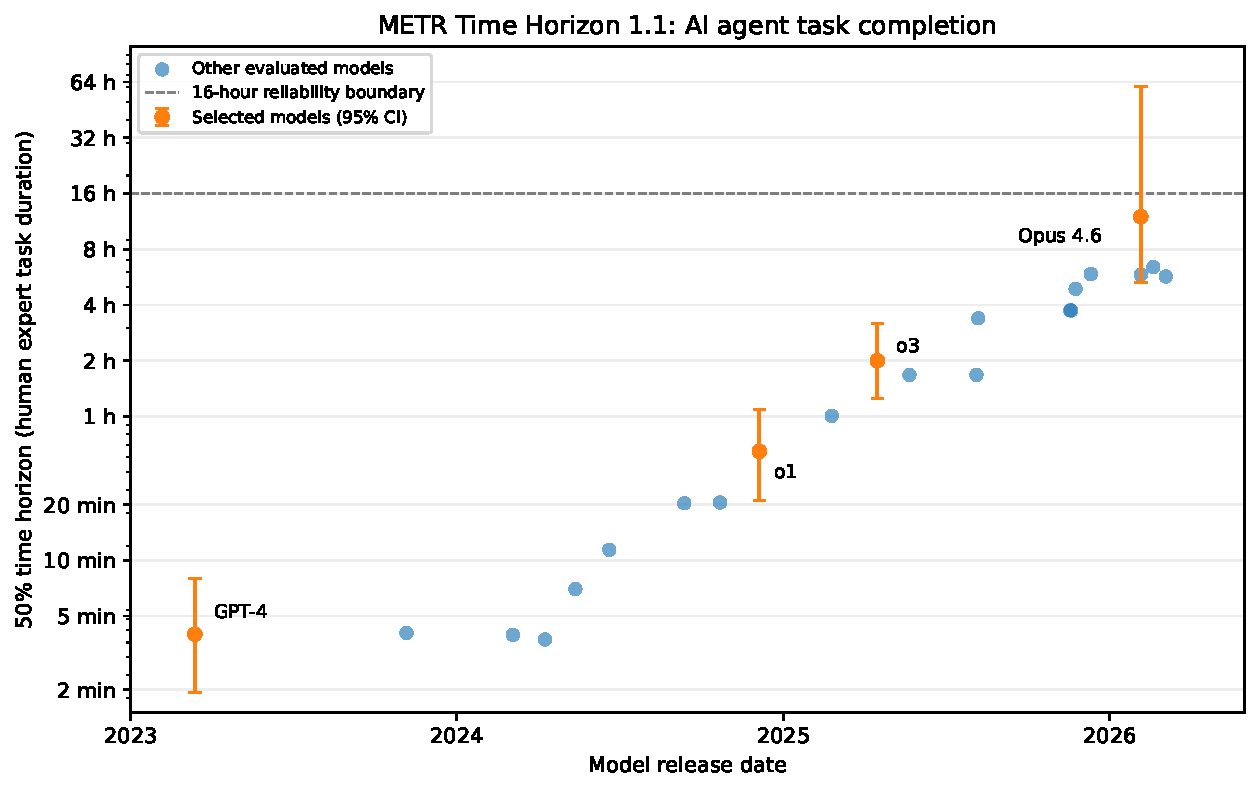
\includegraphics[width=\textwidth, 
alt={Scatter plot showing increasing AI agent task-completion time horizons from 2023 to 2026, with substantial uncertainty in the most capable models.}]{images/metr_time_horizons.pdf}
\caption{Estimated 50\% task-completion time horizons for
AI models released between 2023 and 2026.
The vertical axis represents the duration of tasks measured
by human expert completion time, not the time required
by the AI system. Results are from METR's Time Horizon 1.1
benchmark. Note the logarithmic vertical axis.
Error bars show 95\% confidence intervals for selected models; some extend beyond METR's approximately 16-hour range of reliable estimation.
Point estimates above 16 hours are omitted.
Source: METR \citep{METR2026TimeHorizons}.}
\label{fig:metr_horizon}
\end{figure}

%\input eci

\FloatBarrier
\subsection{AI in Scientific Research}

AI systems have demonstrated capabilities that extend well beyond generating text and images. In mathematics, a 2026 OpenAI reasoning model disproved a longstanding conjecture in discrete geometry; mathematicians subsequently examined the result \citep{OpenAI2026Geometry}.
In biology, the specialized AI system \href{https://alphafold.com/}{AlphaFold} has substantially advanced protein structure prediction \citep{Jumper2021AlphaFold}, and its public database now contains predicted structures for more than 200 million protein sequences \citep{Varadi2024AlphaFoldDB}. AlphaFold 3 extends these capabilities to molecular complexes involving proteins, nucleic acids, and other molecules \citep{Abramson2024AlphaFold3}. These achievements illustrate how AI can contribute to scientific discovery, although the methods, degree of human involvement, and requirements for independent verification differ substantially among applications. Predicted molecular structures may still require experimental validation.

In November 2026, Levent Alpöge, a mathematician at Anthropic,
announced that, working with Claude, he had found a proof of the
Riemann hypothesis, an open problem since 1859
\citep{Alpoge2026RH}. Rather than write a conventional paper, he
released the proof as roughly 17 million lines of code in the
Lean proof assistant. The next day, the Lean FRO and the Mathlib
Initiative issued a joint statement expressing full confidence
that the formal proof is correct, after independent checks
confirmed that the code compiles and that the theorem it proves
matches the standard formal statement of the hypothesis
\citep{LeanFRO2026RH}. Developing an explanation that
mathematicians can read and understand remains an ongoing task.
The episode illustrates this document's central theme: the result
was accepted not because it sounded convincing, but because it
could be checked independently.

\subsection{Future Possibilities}

Continued advances could enable AI systems to contribute increasingly to scientific research, software development, and the design of new AI systems. AI is already being used to assist AI research and development \citep{Anthropic2026RSI}.

\paragraph{Recursive Self-Improvement (RSI)}
Recursive self-improvement refers to a process in which improvements to an AI system increase its ability to make further improvements. Such processes can be considered along a spectrum, from limited feedback loops in which AI assists in improving components of its own operation, to more autonomous systems capable of repeatedly improving their own capabilities. Some bounded forms of iterative improvement have been demonstrated, but sustained, broadly autonomous recursive self-improvement remains an open possibility. Its feasibility and potential rate are uncertain \citep{StanfordHAIRSI,Anthropic2026RSI}.

\paragraph{Artificial General Intelligence (AGI)} is a term commonly used to describe AI systems capable of performing a broad range of intellectual tasks at a level comparable to, or exceeding, human capabilities. There is no universally accepted definition of AGI, and consequently no universally agreed criterion for determining when it has been achieved \citep{StanfordHAIAGI}.

AGI describes a proposed breadth of capabilities, whereas RSI describes a possible process of improvement. Both concepts feature prominently in discussions of AI's future, but predictions about their development and consequences remain uncertain.

\section{Limitations and Critical Evaluation}\label{sec:limitations}

\subsection{Task Dependence and Limits of Generalization}

The capabilities of an AI system depend on more than the
underlying model. They also depend on the information
available to the system, the tools it can use, and the
tasks it has been designed to perform. For example, a
large language model may generate computer code, but
an application equipped with a Python interpreter can
also execute that code and analyze the results.
Similarly, access to external databases or search
tools can extend a model's capabilities beyond the
information acquired during training. 
In the Chicago ozone example, the useful output is not simply a persuasive account: it is a traceable analysis with identifiable observations, documented instrument and averaging details (such as detector type, calibration status, and sampling frequency), and reproducible calculations.

Contemporary AI systems demonstrate a wide range of
capabilities, including recognizing patterns, processing
natural language, generating text and images, writing
computer programs, analyzing data, and performing
multistep tasks. Their performance, however, varies
considerably across applications and subject areas.
Success on a particular task or standardized benchmark
does not necessarily imply comparable performance in
other contexts \citep{Bommasani2021,NIST2024GenAI}.

\subsection{Why AI Systems Can Produce Incorrect Results}

AI-generated information can be incorrect or misleading for
several reasons, including hallucinations, biases in training
data, and limitations on the information available to a model.

\paragraph{Hallucinations}
A model learns to produce plausible continuations, but plausibility
is not the same as factual verification. A citation may have the
familiar form of an author, title, journal, and date without
corresponding to a real article. The history professor might
receive a convincing quotation attributed to Robespierre that
cannot be found in an authentic source. These are examples of
\emph{hallucinations}: generated claims that appear credible but
are incorrect or fabricated. The generation process by itself
does not check each claim against evidence. Verification tools
and retrieved sources may help, but their results also require
scrutiny \citep{Ji2023Hallucination,NIST2024GenAI}.

\paragraph{Training Bias}
AI models learn from datasets that may contain
systematic biases, omissions, and unequal
representation of different populations or
perspectives. These characteristics can influence
their outputs, producing systematic distortions
even when individual statements appear plausible
\citep{Bender2021Parrots,NIST2024GenAI}.

\subsection{Limitations on Available Information}

\paragraph{Temporal Knowledge Limitations}
A \textbf{training cutoff} describes the most recent information
included in a particular stage of model training. A model may therefore
lack current information unless additional training or tools supply it.
For the ozone question, current EPA measurements must be obtained and
examined rather than assumed to be encoded in the model's parameters.
The same issue arises when an education professor asks about a recently
revised curriculum standard or a business professor investigates the
latest financial filings.

This is often discussed in terms of a model's
\emph{knowledge cutoff}. Access to current information
through search tools or external databases can mitigate
this limitation, but the retrieved information and its
interpretation must still be evaluated.

\paragraph{Context Windows}
The \textbf{context window} is the limited amount of information
that a model can process in a given interaction, including instructions,
conversation history, and supplied excerpts. A lengthy document may
exceed the available window, and a model can overlook relevant details
even when they fit. An application may compensate by selecting or
retrieving portions of a document rather than supplying all of it at once.

\subsection{Reliability and Human Oversight}

The capabilities of an AI system should not be confused
with its reliability. A model may be capable of producing
a sophisticated historical interpretation, scientific
analysis, or business forecast without consistently
producing correct results. Moreover, performance on
one task does not necessarily predict performance on
another.

The same principle applies beyond the two recurring examples.
An education professor evaluating a lesson-plan suggestion must check
its fit to a particular learner population and instructional goal.
A business professor reviewing an AI-generated market forecast must
inspect its assumptions and sources, even if the arithmetic is correct.

\paragraph{Interpretability}
It is natural to assume that an AI system's reasoning can be
inspected to determine why it produced a particular answer.
Although the computations performed by a neural network can be
examined, reconstructing a complete, human-understandable
explanation for a particular output is generally not possible
with current methods. Researchers have made progress in
identifying features that models represent and in tracing some
of the pathways connecting them, but such analyses remain
partial \citep{Lindsey2025Biology}. As noted in
Section~\ref{sec:inference}, explanations or reasoning text that
a model provides are themselves generated outputs, not direct
records of its internal computation. Regardless of
interpretability, the reliability of AI outputs must be
established by checking claims, sources, and calculations
\citep{NIST2023AIRMF}.

The distinction between generating information and taking
action has important implications for reliability, security,
and accountability. An incorrect answer from a chatbot
may misinform a user; an incorrect action by an agent
could modify records, disclose confidential information,
or affect other people.

\paragraph{Prompt Injection}
Agents that read web pages, email, or documents introduce a
distinctive security risk. Text encountered during a task may
contain instructions written to manipulate the agent, such as
a web page with hidden text directing it to disclose
information or take an unintended action. Because external
material is incorporated into the model's context, an agent may
treat instructions embedded in that material as authoritative
rather than as content to be processed. This vulnerability,
known as \emph{prompt injection}, is a practical reason to limit
the information and actions available to an agent and to require
human approval for consequential steps
\citep{Greshake2023Injection,NIST2024GenAI}.

Consequently, effective use of AI agents requires
consideration of the actions they are authorized to
perform, the information they can access, and the
circumstances under which human approval should be required.

These distinctions are especially important when AI
systems are used for consequential tasks. The degree
of human oversight required depends on the nature of
the task, the system's demonstrated reliability, and
the consequences of an error \citep{NIST2024GenAI}.

\paragraph{Responsible AI} is a broad term for approaches intended to ensure that AI systems are developed, deployed, and used in ways that are reliable, safe, accountable, and consistent with applicable ethical and legal principles. Common considerations include transparency, privacy, fairness, security, and human oversight. Different organizations and frameworks may emphasize these considerations differently \citep{NIST2023AIRMF}.


\subsection{Practical Verification of AI Outputs}

Reliance on AI does not excuse errors. Faculty, staff,
and students remain responsible for the accuracy of
information they use or present, regardless of whether
AI tools assisted in producing it.

Different limitations call for different verification practices.
Check factual claims, quotations, and scholarly references
against original sources; examine whether evidence and relevant
perspectives are adequately represented; verify that information
is current; reproduce calculations independently; and test
AI-generated code. For consequential work, seek appropriate
subject-matter review \citep{Ji2023Hallucination,Bender2021Parrots,NIST2024GenAI,Kasneci2023Education}.

\paragraph{Limitations of AI-Text Detection}
AI-text detectors are imperfect and may have unequal
false-positive rates; they should not be treated as
conclusive evidence of misconduct \citep{Liang2023Detectors}.
A more informative exercise is to audit an AI-generated
literature summary for invented or misrepresented references,
checking its claims against the cited sources.

\paragraph{A Tale of Two Queries Revisited}

Without access to external sources, the history professor's
assistant may generate its explanation of the French Revolution
from patterns learned during training. It need not have consulted
historical documents, so quotations, citations, and factual
claims still require checking.
The ozone assistant may instead
retrieve actual EPA monitoring data and perform calculations
with external tools. Even then, choosing an appropriate measure of ozone and accounting for detector types and calibration, sampling frequency and data averaging, seasonal variation, and changes in monitoring coverage require informed scientific judgment.
In either case, the crucial question is not simply whether
the response sounds convincing, but what information and methods
the system actually used and how its conclusions can be checked.

\section{Further Reading and Resources}

The following resources provide additional background on AI technologies, capabilities, and limitations. They differ in technical depth and intended audience, and several are updated periodically as the field develops.


\paragraph{Stanford HAI -- Artificial Intelligence Index Report (2026)}
A comprehensive, data-driven annual review of technical progress, adoption, investment, and societal developments. Excellent for readers who want to understand how quickly the field is changing \citep{StanfordHAI2026Index}.

\paragraph{Bommasani et al. -- On the Opportunities and Risks of Foundation Models (2021)}
A foundational academic treatment of foundation models, their capabilities, limitations, and broader implications. More technical than the AI Index \citep{Bommasani2021}.
  
\paragraph{NIST -- AI Risk Management Framework (2023)}
  An authoritative framework for understanding reliability, transparency, accountability, and other characteristics of trustworthy AI systems \citep{NIST2023AIRMF}.

\paragraph{OECD -- Explanatory Memorandum on the Updated OECD Definition of an AI System (2024)}
  An accessible reference for understanding how AI systems are defined and why the boundaries of the term can be difficult to establish \citep{OECD2024AIDefinition}.

\clearpage  
\section{Afterword: Reflections on Writing with AI}\label{sec:afterword}

The process of writing this paper illustrated both the capabilities and limitations of generative AI.
Drafting definitions of common terminology is a task AI models perform as well as---and often better than---a human writer. They are certainly able to do this faster.
AI models are also able to provide correct, detailed explanations of the mathematics behind neural networks and
gradient descent, although those details were not addressed in this manuscript.  Likewise, they can
describe standard aspects of AI development quite capably.
Generative AI was less useful in the framing of the document, although it continued to excel at
identifying language in a draft that needed improvement and suggesting alternative text.
AI models struggled most to identify gaps in explanations and to evaluate the document's pedagogy.
However, once these gaps and missing elements were flagged, AI models
were able to recognize the issues and to suggest helpful revisions.

As of November 2026, I do not think AI could have produced a document like this independently.
While I believe it would have been possible to achieve a result of comparable quality without AI assistance,
it would have required a much greater investment of time---perhaps an order of magnitude more.
For works of this scope, AI's greatest contributions may be not to replace expertise or judgment,
but to make their application far more efficient.

%\nocite{*}
\bibliographystyle{plainnat}
\bibliography{ai}

\end{document}

